\chapter{Methods}

The eartgEngineGrabR package provide an interface of R and the EE to acquire remote sensing data in R. This interface should enable the user to select from some data sets, choose a temporal and spatial resolution and send a request to the EE servers to process and export the data to the user's local machine. The earthEngineGrabR is supposed to work as a foundation that eases further extensions.

The base functionality of the earthEngineGrabR is: 
\begin{itemize}
	\item Uploading vector data to earth engine
	\item Choose from a list of data product
	\item Provide extensive control over the aggregation corresponding to the shape, temporal- and spatial-resolution
	\item Export the data products from EE and import the data into R
	\item Manage the dependencies and authentications to the involved API's
\end{itemize}

The package consists of two functions \mbox{\texttt{ee\_grab()}} and \mbox{\texttt{ee\_grab\_init()}}. The \texttt{ee\_grab\_init()} function handles authentications and the installation of additional dependencies necessary for the earthEngineGrabR package to work. The \texttt{ee\_grab()} function controls the acquisition of the remote sensing data from EE.

First, the data section gives an overview of the data temporarily accessible through the earthEngineGrabR. 
The next section introduces the general design and functionality that the package provides during the acquisition process. The section covers how the \texttt{ee\_grab()} function can select, filter, aggregate and retrieve the requested data, while the emphasis lies on the design workflow and arguments of the function.
The following section introduces the technical framework that enables the interface of R and the EE, while the focus in on the technical side in \texttt{ee\_grab()} function call.
The last section covers the necessary dependencies and authentications processes handled by the \texttt{ee\_grab\_init()}.

\section{Available data products}

The main objective of the current version of the earthEngineGraR package is to develop a stable interface of R and the EE to retrieve data in a user-specific form. Therefore the temporally available data is still limited to a selected list of data products, that should illustrate the diversity of the EE data catalogue (see table \ref{data}). In the further development of the earthEngineGrabR package, this list will be extended.

\begin{table}[h]
	\begin{tabularx}{\textwidth}{|l|l|X|X|X|}
		\hline
		\textbf{data source} & \textbf{data product} & \textbf{spatial} & \textbf{temporal} & \textbf{availability}\\
		\hline
		
		MOD44B.051 & Tree-cover  & 30 m & yearly & 2000–2015 \\
		
		& Non-tree cover  & 30 m & yearly & 2000–2015 \\
		
		& Non-vegetation  & 30 m & yearly & 2000–2015 \\
		
		JRC SW  & Distance to SW & 30 m & yearly & 1984–2015 \\
		
		CHIRPS & Precipitation & 0.05$^\circ$ & yearly & 2000–2015\\
		
		SRTM & Elevation  & 30 m & single & 2000\\
		& Slope  & 30 m & single & 2000\\
		
		Oxford MAP & Accessibility to cities  & 0.01$^\circ$ & single & 2015\\
		
		& Friction surface  & 0.01$^\circ$  & single & 2015\\
		
		\hline
	\end{tabularx}
	\caption{Data products with temporal coverage, temporal- and spatial-resolution available in the earthEngineGrabR}
	\label{data}
\end{table}

In the following, I distinguish between a data source of the remote sensing data, that represents the primary source, for example, the Modis MOD44B.051 Terra Vegetation Continous Fields (VCF) and the derived data product: percent tree cover. In the earthEngineGrabR, the user requests remote sensing data as specific data products. A data product always represents one band of the source satellite image and one environmental variable like percent tree cover, distance to surface water or slope.
The variables vary in temporal and spatial resolution dependent on the data product they are derived from. 

To access land cover, the MOD44B.051 Terra VCF product with a yearly temporal resolution and a 250 m spatial resolution is used. The data set provides a sub-pixel-level representation of surface vegetation cover, designed to continuously represent earth's terrestrial surface as a gradient of three essential surface cover components: percent tree cover, percent non-tree cover and percent bare. The data set is generated using monthly composites of Terra Modis 250 m and 500 m Land Surface Reflectance data (\cite{hansen2006vegetation}).

The Joint Research Center (JRC), Water Classification History, is a data set, produced in collaboration with the European Commission and Google. 
The data set provides a pixel-wise classification of surface water generated using, 3,066,102 scenes from Landsat 5, 7 and 8 acquired between 1984 and 2015. Each pixel was individually classified into water and non-water. The data comes in an original monthly temporal resolution and an aggregated yearly resolution. In the earthEngineGrabR, the aggregated yearly water classification data is used, providing a pixel-wise classification of seasonal water, permanent water and not water (\cite{pekel2016high}). To convert this information in an ecological context, the data is further processed to receive the distance to surface water (SW) product for each pixel. To compute the distance permanent and seasonal water are merged. Therefore the distance refers to permanent and seasonal water.

To provide topographic products, the Shuttle Radar Topography Mission (SRTM) of NASA acquired in 2007 with a spatial resolution of 30 m, is used. While the SRTM dataset provides elevation in meters, the slope product is additionally processed in EE (\cite{farr2007shuttle}). 

To account for socio-economic variables the recently published Oxford MAP datasets of Accessibility to Cities for 2015 and Global Friction Surface for 2015 both with a spatial resolution of 0.01$^\circ$, what corresponds to approximately 30 m, are used. The global Friction Surface map estimates land-based travel speed for land pixels in the year 2015, and the global Accessibility map estimates land-based travel time to the nearest densely-populated area for the year 2015. Both datasets were produced through a collaboration between the Univerity of Oxford Malaria Atlas Project (MAP), Google and the European Union JRC (\cite{weiss2018global}).
To produce the maps, the first time a global-scale combination of Open Street Map data and Google roads dataset was used, extended with datasets for topographic conditions, land cover types and national borders.
For the Friction Surface map, these underlying datasets were used to calculate travel speed regarding time to cross each pixel, with the fastest travel mode intersecting the pixel being used to determine the speed to travel in that pixel. The travel speed is in minutes required to travel one meter. The Accessibility map is produced by using the Friction Surface map in combination with a least-cost-algorithm, which calculates the travel time in minutes for each pixel to the nearest city. Cities were determined by using data from the Global Human Settlement Project.  

The Climate Hazard Group InfraRed Precipitation with Station Data (CHIRPS) is a global rainfall data set with a daily temporal resolution and 0.05$^\circ$ spatial resolution (approximately 150 m) (\cite{funk2015climate}). In the earthEngineGrabR, the CHIRPS daily (version 2.0 final) is utilised, an aggregated version of the daily CHIRPS dataset, with a temporal resolution of 1 days.

For consistency, the data products that have a high spatial resolution like CHIRPS and JRC are only available between 2000 and 2015. This way, there is one corresponding period most data is available in.

\section{Design and functionality of the \\ data manipulation}

As was described in the introduction, the necessary preprocessing of the remote sensing data is an integral part of the data acquisition process. In the earthEngineGrabR, the complete integration and aggregation of the data are outsourced to EE.
Instead of downloading the raw raster data the package provides control to filter and aggregate selected data products according to a given target. This processing allows retrieving the data products in a specific, user-defined format. The user specifies a data product with a corresponding time interval and a temporal reducer, a spatial reducer and a target. 

A data product in the earthEngineGrabR is specified with a earth engine data product-function. Each function specifies one particular data product with the corresponding parameters. The name of the function is \texttt{eeProduct\_ } followed by the source of the data products, underscore the name of the data product. For example: \texttt{eeProduct\_modis\_treeCover()}. The output of the function is simply an object of the class list that specifies the parameters of the requested data product. To use a function, that produces the required parameters instead of committing a list or a vector with the listed parameter, holds several advantages illustrated in the result section.

In the EE a reducer is a way to aggregate data over space and time. In the earthEngineGrabR, there are implementations for simple statistics such as computing the mean, modal, maximum, and minimum value. The temporal reducer aggregates the data over time and the spatial reducer aggregates the data over a region defines by the target. 
The target is defined by vector data, where the spatial extent of the features define the region the spatial reducer is applied over (figure \ref*{Workflow}).

\begin{center}
	\begin{figure}[h]
		\begin{center}
			\includegraphics[width=15cm]{images/processing_flow2-cropped.pdf}
			\caption{Function design and the data manipulation workflow of the \texttt{ee\_grab()} function}
			\label{Workflow}
		\end{center}
	\end{figure}
	% \vskip 2em%
\end{center}

Figure \ref{Workflow} shows the basic processing flow to acquire the modis-tree-cover product for a defined time interval and a specific region. First, the data product is selected, with the corresponding data product function. If the data has a temporal resolution, the time interval as the temporal reducer is set inside the data product function. The time interval is used to filter the collection of the source data set. The images passing the filter are reduced to one image with the given temporal reducer. Next, for each region of the reduced image, which overlaps with a feature in the target vector data, a reducer is applied, and a statistic is computed. This enables the user to temporally and spatially aggregate the remote sensing data in a strongly user specific and flexible approach. The final data is returned as vector data.
The output of the \texttt{ee\_grab()} function is an object of class sf. The sf package provides a convenient approach to work with vector data in R and tries to succeed the widely used sp package in the future (\cite{sf}). An sf object is a data.frame with an additional geometry list-column, what strongly simplifies manipulating an sf object by filtering, selecting or summarising. 
During this entire processing flow, the size of the data is massively reduced, while the data is converted from a large remote sensing datasets in raster format to highly flexible and small vector data. The reasons to use vector data instead of raster data and the corresponding advantages are explained in the discussion.


\section{Technical framework for the interface of R and Earth Engine}

To enable R users to request and download data from EE, the package combines multiple tools like the programming languages R, Python, as well as multiple web services provided by Google such as the Fusion Tables, Google Drive and the EE. While Google Drive is a general file sharing and storage service for all kinds of files, Google Fusion Table is specifically designed to manage tabular data and enables to upload, manipulate, visualise and share small amounts of data online.

Each tool performs a specific task. In R, the user specifies the requested data and initialises all further processes. In Python, the actual request is generated and sent to EE. Because EE can import Fusion Tables, the Google Fusion Table is used to upload local vector data to EE. The EE performs all data processing and exports the data to Google Drive wherefrom it is downloaded and imported into R. 

\begin{center}
	
	\begin{figure}[h]
		\begin{center}
			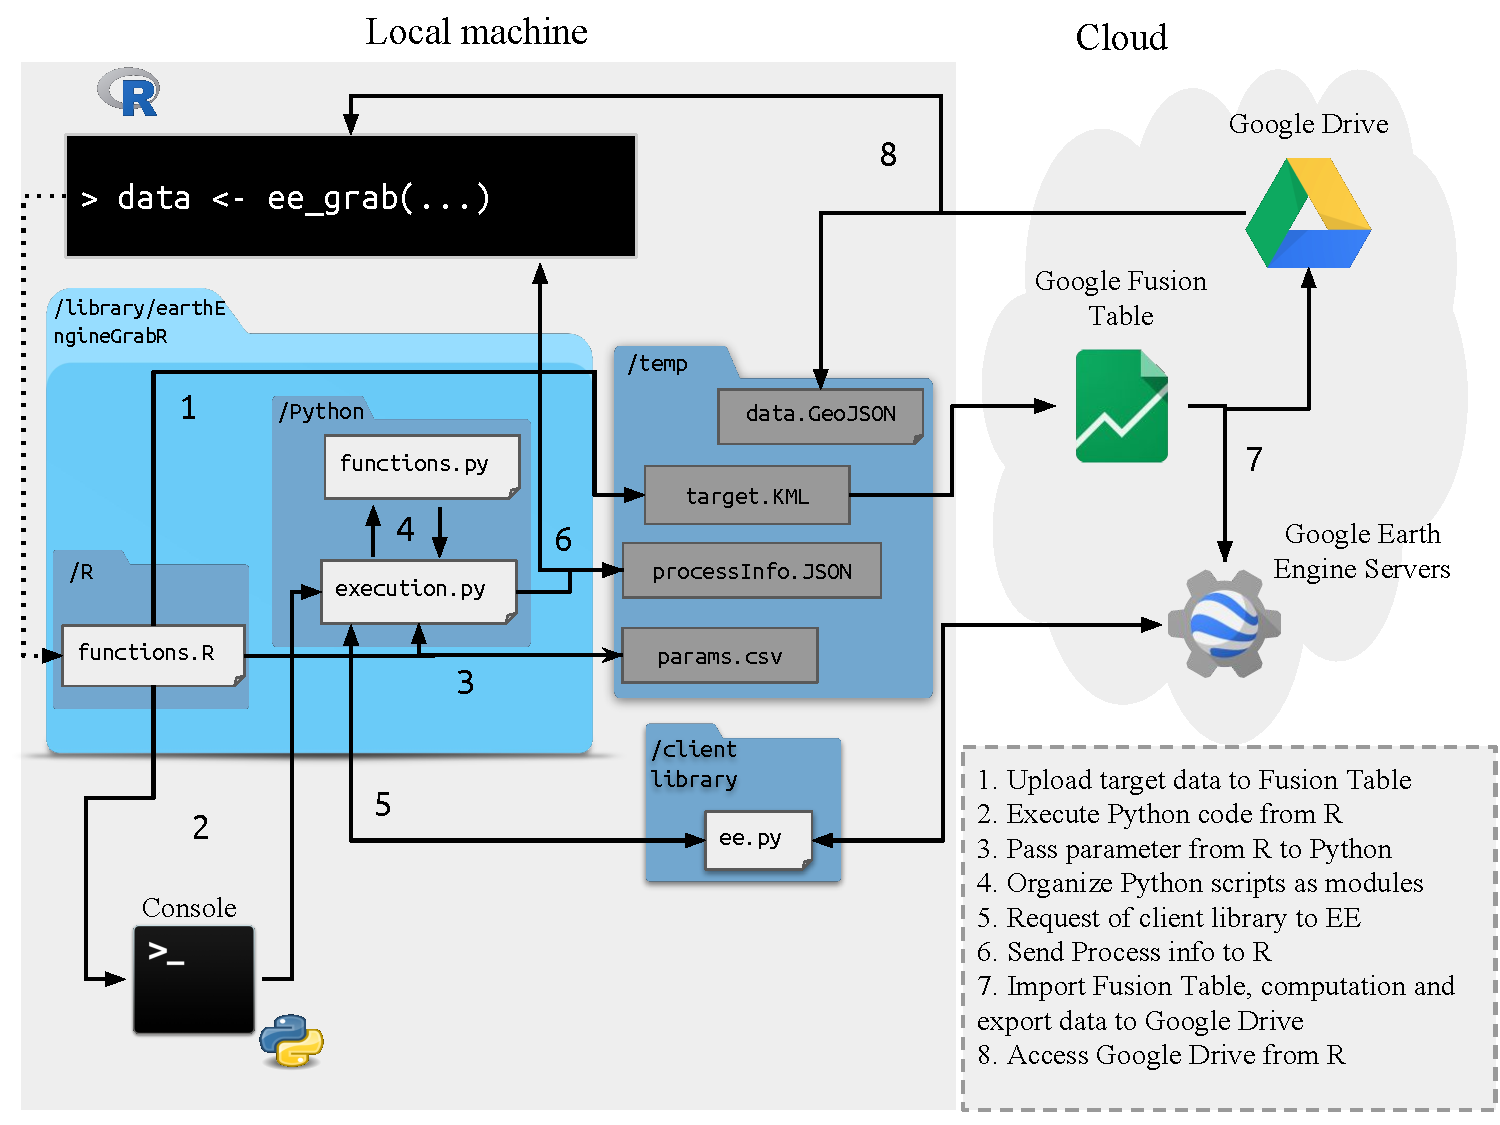
\includegraphics[width=15cm]{images/processing_flow_big.pdf}
			\caption{Internal processing flow of the \texttt{ee\_grab()} function call.}
			\label{processingFlow}
		\end{center}
	\end{figure}
	% \vskip 2em%
\end{center}

In the following an internal processing flow of the \texttt{ee\_grab()} function is described (see figure \ref{processingFlow}).
At the beginning of the function call, the target vector data is uploaded as Fusion Table (1). Next, Python code is executed from R via the system console (2). 
Following, parameters are passed from R to Python via a flat file (3). Python code is organised as modules and devided in execution script and function script (4). The EE client library translates the execution scripts into a request, sends the request to EE  and reseved a response (5). The response containing process info is passed to R via a flat file (6). EE processes the request by import the Fusion Table, perform the requested computation and export the data to Google Drive (7).
Finally Google Drive is accessed from R and the data are downloaded and imported into R subsequently (8).

If installed, the eartEngineGrabR R library is located in a default library folder for all R libraries. In the eartEngineGrabR folder, there is R folder, containing an R script, which defines all R functions used in the package. Furthermore, there is an additional Python folder containing Python scripts divided into execution scripts and function scripts. The function script, again, defines all Python functions. The execution Script, however, is executed from R and uses these functions.

\subsubsection{Upload data to Fusion Table}

To upload the target vector data the Fusion Table driver in the Geospatial Data Abstraction (GDAL) library is used. To execute GDAL from R, R's ability to invoke function calls is applied. This method will be explained in more detail in the following section. GDAL's \texttt{ogr2ogr()}  function handles the upload process, that converts a variety of geo file formats to a Fusion Table. In Fusion Tables, geometries need to be expressed in the World Geodetic System 1984 (WGS84). Therefore the projection of the vector data uploaded as Fusion Table is converted.

\subsubsection{Integration of R and Python}

The EE is accessed with the EE client library for Python. To access EE from R it's necessary to execute Python from R. The integration enable to pass arguments from R to Python and execute Python code from R. Instead of using a Python wrapper for R such as the rPython package, earthEngineGrabR utilizes a simple command line or terminal to execute one language from the other. The \texttt{ee\_grab()} function defined in the R script functions.R, invokes a system call by utilising the command line that executes the python execution script (execution.py) and simultaneously, passes the parameters, to the execution scripts by using a flat file (2). 

\begin{center}
	\begin{figure}[h]
		\begin{center}
			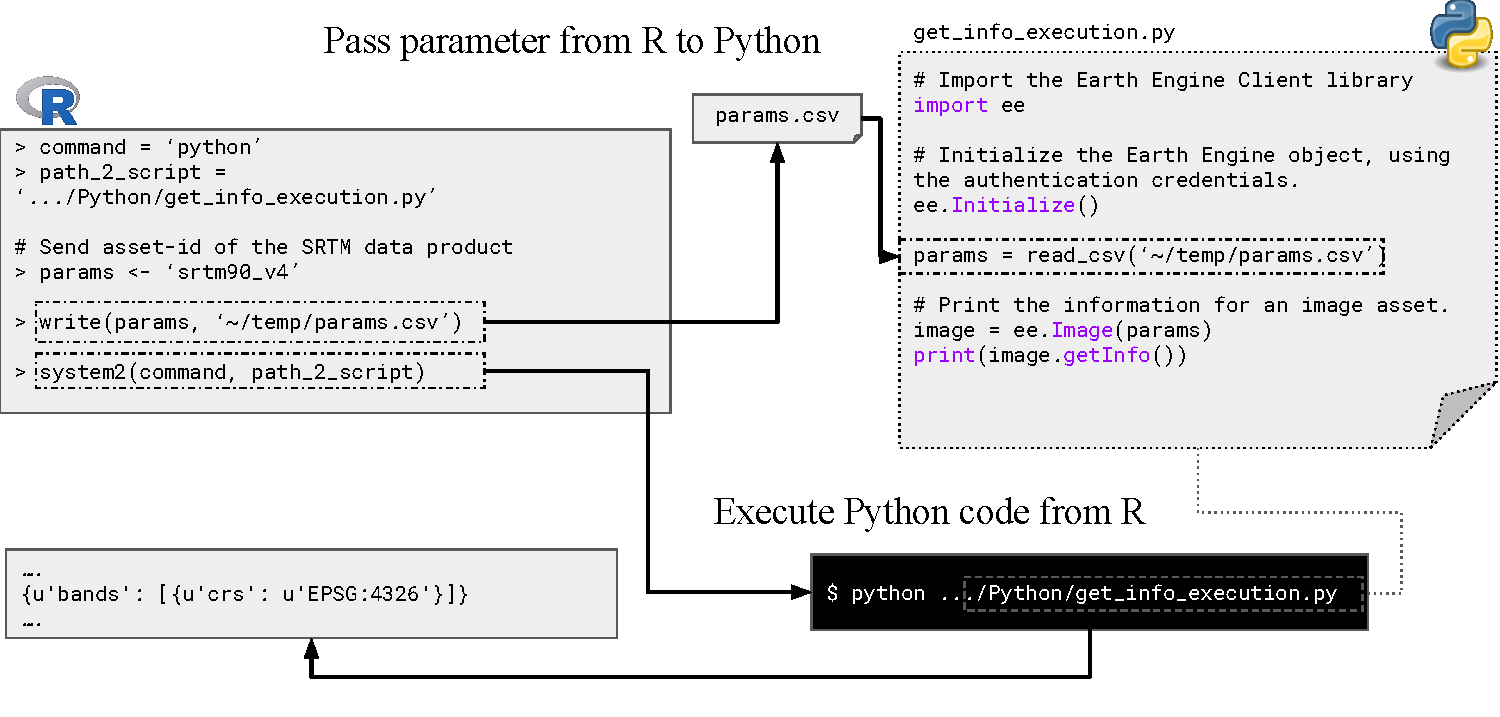
\includegraphics[width=15cm]{images/concole_connection_big-cropped.pdf}
			\caption{Example of utilizing the console to execute a Python script from R, that requests metadata on the SRTM data set on EE.}
			\label{consoleConnection}			
		\end{center}
	\end{figure}
	% \vskip 2em%
\end{center}


To illustrate this two processes in practice, figure \ref{consoleConnection} shows a simplified code example of how to retrieve metadata of a specified data product from EE in R with the command line as the connection of R and Python. The figure presents how to execute Python code from R and how to pass parameters from R to Python. The left boxes illustrate the R console, the right box the Python execution script and the black box the command line.
In R the \texttt{system2()} function of the base package invoices system commands and additional arguments in all operating systems. 
To run the Python script \texttt{get\_info.py}, the system call simply consists of the command \texttt{python}, to open the Python interpreter and the path to the Python script. The \texttt{system2()} function then produces the system call in the command line shown in the black box and runs the \texttt{get\_info.py} script. To pass parameters from R to Python a flat file connection is used. The Parameter is defined in R, then written to a CSV file and read again into the execution script. In this example, the parameter is the asset-id of the SRTM data set in EE. 
In the Python script \texttt{get\_info\_execution.py}, first, the EE client library is imported and initialised with the authentication credentials then the parameters are imported. To load the SRTM data product from the EE data catalogue, the asset-id is put inside an EE object (\texttt{ee.Image()}) specifying an image. To access metadata from this EE object their \texttt{getInfo()} method is called and put inside a \texttt{print()} statement. The output of this script is the output of the print command. This output is formatted in JSON and in the default setting of the \texttt{system2()} function, the output is directly printed to the R console. Although simplified, this example shows the essential integration of R and Python and the approach to pass parameters. 
Instead of a print command, the earthEngineGrabR utilises a export command to initializes the export of the data to Google Drive.

Although it would be possible to send parameters directly over the command line, with an increasing number of parameter, this method becomes confusing and error-prone due to text formatting differences of the command line dependent on the operating system. Therefore the package utilises a flat file connection that provides a reliable method for exchanging parameters independent from the operating system.

\subsubsection{Organize Python code as modules}

All necessary processing of the data in EE is described with the EE client library in Python. To maintain a well-arranged structure, the code is organised like a sub-package, inside the earthEngineGrabR package. There is an execution script, executed with the method described above, that calls functions defined in a Python script (functions.py) (4). The functions script defines all functions necessary for the data manipulation workflow shown in figure \ref*{Workflow}. The functions are organised like independent modules, each describing one process in the processing chain shown in figure \ref*{Workflow}. There are functions for temporal filtering and reduction, spatial reduction and export. The modules take the parameters as function arguments, and this way provide the described control over the requested data.

\subsubsection{Communication of the client library, EE and Google Drive}

The client library consists of objects, which represent placeholders for data types stored on the EE servers, each object has corresponding methods or functions that manipulate this data type. Figure \ref{consoleConnection} showed an example of an EE object for an Image. To perform a computation in EE, the objects and corresponding methods are composed and combined to build a description of the computation the user wants to perform. 

At the moment the script is executed, this description is sent to the EE servers through a Representational State Transfer (REST) API (5). REST is a web service often used to request and modify data on a server through a Hypertext Transfer Protocol (HTTP).
In the context of the EE client library, it refers to using HTTP verbs to retrieve and modify representations of data stored on Google's servers.

In a REST system, resources are stored in a data store. A client sends a request that the server performs a particular action (such as creating, retrieving, updating, or deleting a resource), and the server performs the action and sends a response. In the case of the earthEngineGrabR, the request is: import a specific data product, import a specific Fusion Table, filter a time interval, aggregate over time, aggregate over regions defiend by the Fusion Table and export the generated data to Google Drive (7)

While this is the action of the request that is performed the response of the request is to send info about the export process (6). This process info includes metadata of the exported object and whether the export was successful or not. To pass this info to R again a flat file is used, the info is written to disk as a JSON file and afterwards imported into R. The last step in the processing chain is to access Google Drive from R and first download and next import the data into R (8). To access Google Drive from R, the googledrive R package is used. The googledrive package enables selection and download of specific files stored on the users Google Drive account. To identify the files to download, the metadata included in the retrieved process info is used. First, the data is downloaded in the temp folder that corresponds to the current working directory and if available on disk imported into R.

\subsubsection{Parallel processing of data products}


To process multiple data products in a \texttt{ee\_grab()} function call, each data product is processed in an individual request to the EE servers. While the upload of the target vector is performed only once, the remaining seven processes of the processing flow in figure \ref{processingFlow} are iterated for each data product. This approach allows the parallel processing of the data products. The individual requests for the data products, generated by the EE client library in Python, all end with a command to export the generated data to Google Drive (in figure \ref{processingFlow} shown as green arrows with number 7). However, the request must not wait until the data is processed and exported to Google Drive. Instead, the request ends with the response of the EE servers, whether EE started the processing. 
This allows requesting the computation of multiple data products at the same time. The exported data products are individually downloaded from Google Drive and finally joined in R.


\section{Organize dependencies and authentications}


The earthEngineGrabR package has several package dependencies in R and Python. While most R dependencies can be handled within the description file of an R package, the Python dependencies need to be manually installed with a package manager like pip. Furthermore, the package connects to several API's, which each require an individual, user-specific, authentication procedure. Therefore, a user-friendly organisation of all requirements of the earthEngineGrabR to work is particularly important. To leave the installation of dependencies and authentications to the user, would significantly hinder the use of the package and make it more cumbersome. 


To simplify the installation and authentication process, the earthEngineGrabR includes a function \texttt{ee\_grab\_init()} that installs Python dependencies and furthermore guides the user through the different authentications. Before using the earthEngineGrabR, the user has to call \texttt{ee\_grab\_init()}. 

\subsubsection{Dependencies}

Table \ref*{dependencies} lists the different dependencies for the earthEngineGrabR and how they are installed. 

\begin{table}[h]
	\begin{tabularx}{\textwidth}{|X|C|C|}
		\hline
		\textbf{library} & \textbf{dependency} & \textbf{installation}  \\
		\hline
		googledrive & R  & description file  \\
		dplyr & R  & description file  \\
		rjson & R  & description file  \\
		sf & R  & not provided  \\
		GDAL & R, Python  & not provided  \\
		google api python client & Python  & setuptools  \\
		pyCrypto & Python  & setuptools  \\
		earthengine-api & Python  & setuptools  \\        
		pandas & Python  & setuptools  \\        
		json & Python  & setuptools  \\        
		\hline
	\end{tabularx}
	\caption{Library dependencies of the earthEngineGrabR and how the installation is handled}
	\label{dependencies}
\end{table}

The dependencies handled by the description file are automatically installed during the installation of the earthEngineGrabR, while the libraries dealt with the setuptools utility are installed with \texttt{ee\_grab\_init()}. The installation of sf and GDAL is not provided and has to be manually installed by the user prior to the use of the earthEngineGrabR.

The earthEngineGrabR depends on a Python version higher 2.7 with Python path set (PYTHONPATH). To ease the installation of the Python dependencies, all dependencies are combined in a new python package (GEE2R), using the setuptools package in Python. The GEE2R Python package can then be installed with the package manager pip. During this installation, all specified python dependencies are installed at once. This process is similar to the use of the description file in R packages. To call pip from R, R's described ability to invoke a system call with the \texttt{system()} or \texttt{system2()} function is used.

\subsubsection{Authentication}

In the earthEngineGrabR, three APIs are used. The EE API, the Google Drive API and the Google Fusiontable API. Each API require an authentification with a valid Google account, and concerning the Google Earth Engine API, a Google account activated for EE use. According to Google, the EE is free for research, education and nonprofit use furthermore results of the analysis performed by the user, as well as new algorithms wrote by the user remain in the property of the user alone (\cite{terms}).
To get access to EE the user has to fill out a form and wait until the request for excess is granted. If the excess is granted the user's Google account activated for excessing EE. For utilising the Google Drive API and Google Fusiontable API, only a valid Google Account is necessary. All API's use the OAuth 2.0 Protocol to manage the authentication process. To send a valid request to one of these APIs, the request needs to be authorised with a valid access token generated with the OAuth 2.0 protocol (\cite{hardt2012oauth}). To manage the OAuth 2.0 protocol and generate these tokens the earthEngineGrabR package uses different approaches depending on how each API is accessed. 

The initial call of the \texttt{ee\_grab\_init()} guides the user through the different authentications. The \texttt{ee\_grab\_init()} function only needs to be called once, and the required authentification tokens are saved and managed independently. 





